
\section{Metodología de desarrollo}
Para la realización del proyecto y su documentación se ha utilizado el {\em Rational Unified Process (RUP)}, junto con el {\em Lenguaje Unificado de Modelado (UML)}. Se ha elegido este sistema ya que es la metodología estándar más utilizada, además de ser un grupo de metodologías que se adaptan muy bien a las necesidades de un producto.

\section{Especificación de requisitos del sistema}
A continuación se enumeran los requisitos funcionales que se consideran fundamentales para el sistema. Éstos serán detallados utilizando casos de uso, describiendo tanto su escenario principal como sus posibles flujos alternativos. Además se detallará cada caso de uso con su diagrama de secuencia correspondiente.


\subsection{Gestión de titulaciones}
 Aquí va el diagrama de casos de uso de la gestión de titulaciones.

\begin{figure}[H] 
  \label{gestion-titulaciones} 
	\begin{center}
    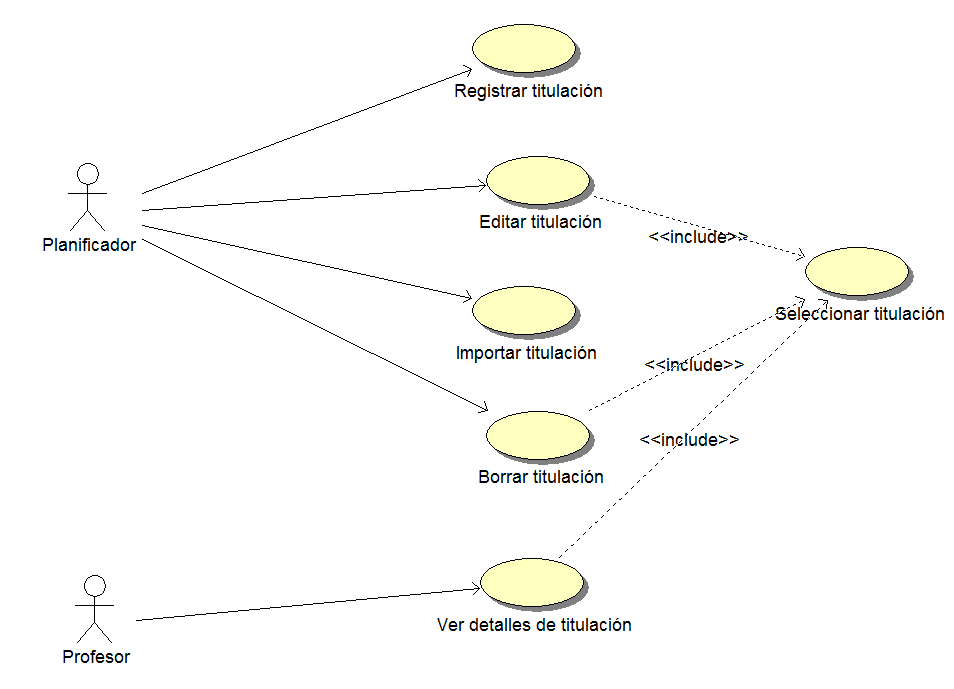
\includegraphics[scale=0.5]{./gestiontitulaciones.png}
  \end{center}
\caption{Diagrama de casos de uso de la gestión de titulaciones}
\end{figure}
\subsubsection*{Caso de uso: Seleccionar titulación}
\label{select_titulacion}
\begin{itemize}
\item{\bf Descripción:} Caso de uso abstracto incluído en otros casos de uso para seleccionar una titulación de una lista de disponibles.
\item{\bf Actores:} Usuario
\item{\bf Precondiciones:} Ninguna.
\item{\bf Postcondiciones:} Se selecciona una titulación para su uso en otra finalidad.
\item{\bf Escenario principal:}
\begin{enumerate}
\item El sistema muestra un listado de las titulaciones disponibles.
\item El usuario selecciona la titulación deseada.
\end{enumerate}
\item{\bf Escenarios alternativos:}
\begin{itemize}
\item[1.a.] No hay ninguna titulación registrada.
\begin{enumerate}
\item El sistema indica el error y el caso de uso finaliza.
\end{enumerate}
\end{itemize}
\end{itemize}



\subsubsection*{Caso de uso: Registrar titulación}
\begin{itemize}
\item{\bf Descripción:} Registra una nueva titulación en el sistema.
\item{\bf Actores:} Administrador.
\item{\bf Precondiciones:} Ninguna.
\item{\bf Postcondiciones:} La titulación queda registrada.
\item{\bf Escenario principal:}
\begin{enumerate}
\item El administrador introduce el código, el nombre y todos los demás datos de la titulación.
\item El sistema comprueba que los datos cumplen el formato.
\item El sistema confirma el alta de la titulación mostrando un mensaje.
\end{enumerate}
\item{\bf Escenarios alternativos:}
	\begin{itemize}
	\item[2.a.] Alguno de los datos introducidos tiene un formato incorrecto.
		\begin{enumerate}
		\item El sistema lo indica mostrando un mensaje de error y se vuelve al paso anterior.
		\end{enumerate}
	\item[2.b.] Falta algún campo obligatorio.
		\begin{enumerate}
		\item El sistema lo indica mostrando un mensaje de error y se vuelve al paso anterior.
		\end{enumerate}
	\item[2.c.] Ya existe alguna titulación con ese código o nombre.
		\begin{enumerate}
		\item El sistema indica el error y se vuelve al paso anterior.
		\end{enumerate}
	\item[*a.] El administrador decide cancelar el registro en cualquier momento, el caso de uso termina. 
	\end{itemize}
\end{itemize}



\subsubsection*{Caso de uso: Editar titulación}
\begin{itemize}
\item{\bf Descripción:} Edita una titulación existente en el sistema modificando sus datos.
\item{\bf Actores:} Administrador.
\item{\bf Precondiciones:} Ninguna.
\item{\bf Postcondiciones:} La titulacion queda modificada en el sistema.
\item{\bf Escenario principal:}
\begin{enumerate}
	\item Se realiza el caso de uso {\em\hyperref[select_titulacion]{Seleccionar titulación}}.
	\item El sistema muestra sus datos actuales, permitiendo su edición.
	\item El administrador modifica los datos.
	\item El sistema comprueba que todos los datos son correctos.
	\item El sistema muestra un mensaje indicando que la edición se ha completado.
\end{enumerate}
\item{\bf Escenarios alternativos:}
	\begin{itemize}
	\item[4.a.] Alguno de los datos tiene un formato incorrecto.
		\begin{enumerate}
		\item El sistema muestra un mensaje de error indicándolo, a continuación se vuelve al paso anterior.
		\end{enumerate}
	\item[4.b.] Falta algún campo obligatorio por rellenar.
		\begin{enumerate}
		\item El sistema muestra un mensaje de error indicándolo, a continuación se vuelve al paso anterior.
		\end{enumerate}
	\item[4.c.] Ya existe alguna titulación con el nombre o código introducidos.
		\begin{enumerate}
		\item El sitema indica el error y se vuelve al paso anterior.
		\end{enumerate}
	\item[*a.] En cualquier momento el administrador decide cancelar la edición, el caso de uso se da por terminado.
	\end{itemize}
\end{itemize}



\subsubsection*{Caso de uso: Borrar titulación}
% Tomar este CU como ejemplo
\begin{itemize}
\item{\bf Descripción:} Borra una titulación del sistema.
\item{\bf Actores:} Administrador.
\item{\bf Precondiciones:} La titulación existe en el sistema.
\item{\bf Postcondiciones:} La titulación queda eliminada del sistema.
\item{\bf Escenario principal:}
	\begin{enumerate}
	\item Se realiza el caso de uso  {\em\hyperref[select_titulacion]{Seleccionar titulación}}.
	\item El sistema muestra un diálogo de confirmación.
	\item El administrador confirma que quiere eliminar la titulación del sistema.
	\item El sistema elimina la titulación.
	\item El sistema muestra un mensaje confirmando que se ha eliminado la titulación.
	\end{enumerate}
\item{\bf Escenarios alternativos:}
	\begin{itemize}
	\item[3.a.] El administrador selecciona que no desea eliminar la titulación.
		\begin{enumerate}
		\item El caso de uso se reinicia.
		\end{enumerate}
	\item[*a.] En cualquier momento el administrador decide cancelar la eliminación.
		\begin{enumerate}
		\item El caso de uso se termina.
		\end{enumerate}
	\end{itemize}
\end{itemize}



\subsubsection*{Caso de uso: Ver detalles de titulación}
\begin{itemize}
\item{\bf Descripción:} Muestra los datos de una titulación en detalle, así como sus asignaturas.
\item{\bf Actores:} Usuario.
\item{\bf Precondiciones:} La titulación existe en el sistema.
\item{\bf Postcondiciones:} Los datos de la titulación se muestran por pantalla.
\item{\bf Escenario principal:}
	\begin{enumerate}
	\item Se realiza el caso de uso {\em\hyperref[select_titulacion]{Seleccionar titulación}}.
	\item El sistema muestra los datos de la titulación y un listado de sus asignaturas si las tiene.
	\end{enumerate}
\item{\bf Escenarios alternativos:}
	\begin{itemize}
	\item[*a.] En cualquier momento el usuario decide cancelar el proceso, el caso de uso se termina.
	\end{itemize}
\end{itemize}





\subsubsection*{Caso de uso: Importar titulación}
\begin{itemize}
\item{\bf Descripción:} Caso de uso para importar titulaciones de forma masiva desde un archivo csv con un formato concreto.
\item{\bf Actores:} Administrador
\item{\bf Precondiciones:} El archivo tiene el formato correcto.
\item{\bf Postcondiciones:} Se crean las titulaciones indicadas en el archivo.
\item{\bf Escenario principal:}
	\begin{enumerate}
	\item El administrador selecciona el archivo.
	\item El sistema comprueba que cada línea tenga el formato correcto.
	\item El sistema crea una titulación por cada línea con los datos indicados en el archivo.
	\end{enumerate}
\item{\bf Escenarios alternativos:}
	\begin{itemize}
		\item[2.a.] Alguna línea no cumple el formato
		\begin{enumerate}
			\item El sistema indica el error y el caso de uso finaliza.
		\end{enumerate}
		\item[2.b.] Ya existe una titulación creada con el mismo identificador.
		\begin{enumerate}
			\item El sistema lo indica y el caso de uso finaliza.
		\end{enumerate}
	\end{itemize}
\end{itemize}



\subsubsection{Gestión de asignaturas}
% Aquí va el diagrama de la gestión de asignaturas
\begin{figure}[H] 
  \label{gestion-asignaturas} 
	\begin{center}
    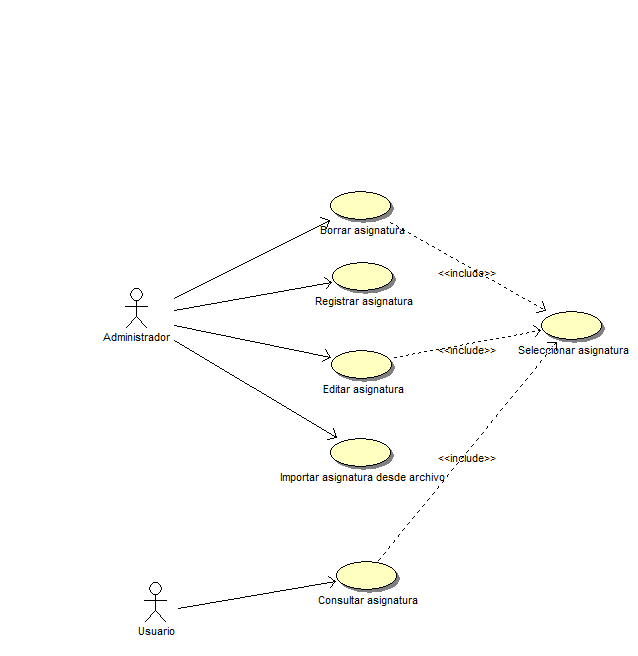
\includegraphics[scale=0.5]{./gestionasignaturas.png}
  \end{center}
\caption{Diagrama de casos de uso de la gestión de asignaturas}
\end{figure}
\subsubsection*{Caso de uso: Seleccionar asignatura}
\label{select_asignatura}
\begin{itemize}
\item{\bf Descripción:} Caso de uso abstracto incluído por otros casos de uso para seleccionar una asignatura del listado de las que tiene disponibles una titulación concreta.
\item{\bf Actores:} Usuario
\item{\bf Precondiciones:} Ninguna.
\item{\bf Postcondiciones:} Queda seleccionada una asignatura para algún fin concreto de otro caso de uso.
\item{\bf Escenario principal:}
	\begin{enumerate}
	\item Se realiza el caso de uso {\em\hyperref[select_titulacion]{Seleccionar titulación}}.
	\item El sistema muestra un listado de las asignaturas disponibles asociadas a la titulación seleccionada.
	\item El usuario selecciona una asignatura de la lista.
	\end{enumerate}
\item{\bf Escenarios alternativos:}
	\begin{itemize}
		\item[2.a.] No hay ninguna asignatura registrada en esa titulación.
		\begin{enumerate}
			\item El sistema indica el error y el caso de uso finaliza.
		\end{enumerate}
	\end{itemize}
\end{itemize}



\subsubsection*{Caso de uso: Registrar asignatura}
\begin{itemize}
\item{\bf Descripción:} Se da de alta una nueva asignatura en el sistema.
\item{\bf Actores:} Administrador.
\item{\bf Precondiciones:} Existe alguna titulación con la que asociar la asignatura.
\item{\bf Postcondiciones:} La asignatura queda registrada en el sistema.
\item{\bf Escenario principal:}
	\begin{enumerate}
 	\item Se realiza el caso de uso {\em\hyperref[select_titulacion]{Seleccionar titulación}}.
	\item El sistema muestra un formulario para introducir los datos.
	\item El administrador introduce el código, el nombre y todos los demás datos de la asignatura.
	\item El sistema comprueba que todos los datos cumplen el formato requerido.
	\item El sistema registra la asignatura y muestra un mensaje confirmándolo.
	\end{enumerate}
\item{\bf Escenarios alternativos:}
	\begin{itemize}
	\item[3.a.] El administrador selecciona que desea tomar los datos de otra asignatura.
		\begin{enumerate}
		\item Se realiza el caso de uso {\em \hyperref[duplicar_asignatura]{Duplicar asignatura}}.
		\end{enumerate}
	\item[4.a.] Alguno de los datos no cumple el formato correcto.
		\begin{enumerate}
		\item El sistema indica el error y se vuelve al paso anterior.
		\end{enumerate}
	\item[4.b.] Falta por rellenar algún campo obligatorio.
		\begin{enumerate}
		\item El sistema indica el error y se vuelve al paso anterior.
		\end{enumerate}
	\item[4.c.] Ya existe alguna asignatura con ese código o nombre.
		\begin{enumerate}
		\item El sistema indica el error y se vuelve al paso anterior.
		\end{enumerate}
	\item[*a.] En cualquier momento el administrador decide cancelar el proceso.
		\begin{enumerate}
		\item El caso de uso se cancela.
		\end{enumerate}
	\end{itemize}
\end{itemize}



\subsubsection*{Caso de uso: Editar Asignatura}
\begin{itemize}
\item{\bf Descripción:} Se modifican los datos de una asignatura existente en el sistema.
\item{\bf Actores:} Administrador.
\item{\bf Precondiciones:} Ninguna.
\item{\bf Postcondiciones:} La asignatura queda modificada en el sistema.
\item{\bf Escenario principal:}
	\begin{enumerate}
	\item Se realiza el caso de uso {\em \hyperref[select_asignatura]{Seleccionar asignatura}}.
	\item El sistema muestra los datos de la asignatura en un formato editable.
	\item El administrador hace las modificaciones que considere necesarias.
	\item El sistema comprueba que los datos modificados cumplen el formato requerido.
	\item El sistema guarda la asignatura y muestra un mensaje confirmándolo.
	\end{enumerate}
\item{\bf Escenarios alternativos:}
	\begin{itemize}
	\item[4.a.] Alguno de los datos no cumple el formato correcto.
		\begin{enumerate}
		\item El sistema indica el error y se vuelve al paso anterior.
		\end{enumerate}
	\item[4.b.] Falta por rellenar algún campo obligatorio.
		\begin{enumerate}
		\item El sistema indica el error y se vuelve al paso anterior.
		\end{enumerate}
	\item[4.c.] Ya existe alguna asignatura con ese código o nombre.
		\begin{enumerate}
		\item El sistema indica el error y se vuelve al paso anterior.
		\end{enumerate}
	\item[*a.] En cualquier momento el administrador decide cancelar el proceso.
		\begin{enumerate}
		\item El caso de uso se cancela.
		\end{enumerate}
	\end{itemize}
\end{itemize}



\subsubsection*{Caso de uso: Borrar asignatura}
\begin{itemize}
\item{\bf Descripción:} Se borra una asingatura del sistema.
\item{\bf Actores:} Administrador.
\item{\bf Precondiciones:} Ninguna.
\item{\bf Postcondiciones:} La asignatura queda eliminada del sistema.
\item{\bf Escenario principal:}
	\begin{enumerate}
	\item Se realiza el caso de uso {\em \hyperref[select_asignatura]{Seleccionar asignatura}}.
	\item El sistema muestra un diálogo de confirmación.
	\item El administrador confirma que desea borrar la asignatura.
	\item El sistema borra la asignatura y muestra un mensaje confirmándolo.
	\end{enumerate}
\item{\bf Escenarios alternativos:}
	\begin{itemize}
	\item[3.a.] El administrador selecciona que no desea eliminar la asignatura.
		\begin{enumerate}
		\item El caso de uso se reinicia.
		\end{enumerate}
	\item[*a.] En cualquier momento el administrador decide cancelar la eliminación.
		\begin{enumerate}
		\item El caso de uso se termina.
		\end{enumerate}
	\end{itemize}
\end{itemize}



\subsubsection*{Caso de uso: Consultar asignatura}
\begin{itemize}
\item{\bf Descripción:} Muestra los datos en detalle de una asignatura.
\item{\bf Actores:} Usuario.
\item{\bf Precondiciones:} Ninguna.
\item{\bf Postcondiciones:} Se muestran los datos de la asignatura por pantalla.
\item{\bf Escenario principal:} 
	\begin{enumerate}
	\item Se realiza el caso de uso {\em \hyperref[select_asignatura]{Seleccionar asignatura}}.
	\item El sistema muestra la información relacionada con la asignatura.
	\end{enumerate}
\item{\bf Escenarios alternativos:}
	\begin{itemize}
	\item[*a.] En cualquier momento el administrador decide cancelar el proceso.
		\begin{enumerate}
		\item El caso de uso se termina.
		\end{enumerate}
	\end{itemize}
\end{itemize}


\subsubsection*{Caso de uso: Importar asignatura desde archivo}
\begin{itemize}
\item{\bf Descripción:} Caso de uso para importar asignaturas de forma masiva desde un archivo csv con un formato concreto.
\item{\bf Actores:} Administrador
\item{\bf Precondiciones:} El archivo tiene el formato correcto.
\item{\bf Postcondiciones:} Se crean las asignaturas indicadas en el archivo.
\item{\bf Escenario principal:}
	\begin{enumerate}
	\item El administrador selecciona el archivo.
	\item El sistema comprueba que cada línea tenga el formato correcto.
	\item El sistema crea una asignatura por cada línea con los datos indicados en el archivo.
	\end{enumerate}
\item{\bf Escenarios alternativos:}
	\begin{itemize}
		\item[2.a.] Alguna línea no cumple el formato
		\begin{enumerate}
			\item El sistema indica el error y el caso de uso finaliza.
		\end{enumerate}
		\item[2.b.] Ya existe una asignatura creada con el mismo identificador.
		\begin{enumerate}
			\item El sistema lo indica y el caso de uso finaliza.
		\end{enumerate}
	\end{itemize}
\end{itemize}


\subsubsection{Gestión de cursos}
\begin{figure}[H] 
  \label{gestion-cursos} 
	\begin{center}
    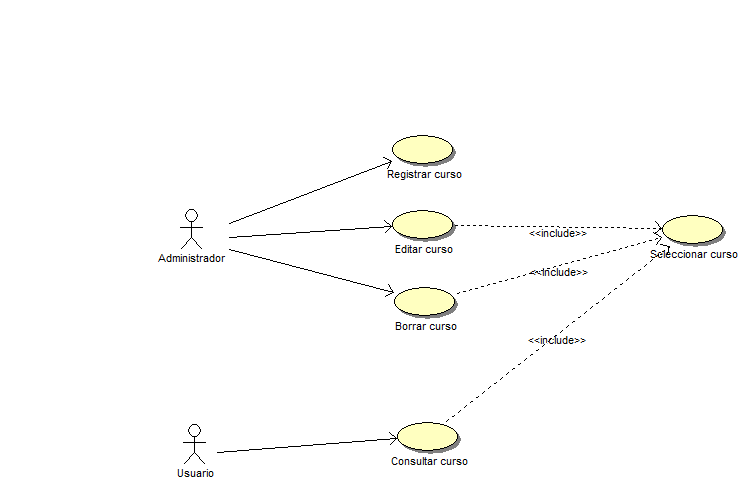
\includegraphics[scale=0.5]{./gestioncursos.png}
  \end{center}
\caption{Diagrama de casos de uso de la gestión de cursos}
\end{figure}

\subsubsection*{Caso de uso: Seleccionar curso}
\begin{itemize}
\item{\bf Descripción:} Caso de uso abstracto que es incluído en otros casos de uso.
\item{\bf Actores:} Usuario.
\item{\bf Precondiciones:} Ninguna.
\item{\bf Postcondiciones:} Queda seleccionado un curso para su uso con algún fin.
\item{\bf Escenario principal:}
	\begin{enumerate}
	\item El sistema muestra un listado con los cursos disponibles.
        \item El usuario selecciona un curso.
	\end{enumerate}
\item{\bf Escenarios alternativos:}
	\begin{itemize}
	\item[1.a.]No hay ningún curso registrado en el sistema.
	  \begin{enumerate}
	  \item El sistema indica el error y el caso de uso finaliza.
	  \end{enumerate}
	\end{itemize}
\end{itemize}




\subsubsection*{Caso de uso: Registrar curso}
\begin{itemize}
\item{\bf Descripción:} Se da de alta en el sistema la configuración de un nuevo curso.
\item{\bf Actores:} Administrador.
\item{\bf Precondiciones:} Ninguna.
\item{\bf Postcondiciones:} Queda registrado en el sistema el curso.
\item{\bf Escenario principal:}
  \begin{enumerate}
  \item El administrador introduce los datos de configuración del curso, incluyendo fecha de inicio y final de curso.
  \item El sistema comprueba que los datos sean correctos.
  \item El sistema informa de que el curso ha sido registrado con éxito.
  \end{enumerate}
\item{\bf Escenarios alternativos:}
  \begin{itemize}
  \item[2.a.] Alguno de los datos introducidos no cumple el formato correcto.
    \begin{enumerate}
    \item El sistema indica el error y se vuelve al paso anterior.
    \end{enumerate}
  \item[2.b.] Ya existe un curso registrado que empieza o termina en el mismo año que el introducido.
    \begin{enumerate}
    \item El sistema indica el error y se vuelve al paso anterior.
    \end{enumerate}
  \item[2.c.] Los años introducidos de inicio y fin del curso no son consecutivos.
    \begin{enumerate}
    \item El sistema indica el error y se vuelve al paso anterior.
    \end{enumerate}
  \item[2.d.] Alguna de las fechas de exámenes introducidas no están comprendidas entre la duración del curso.
    \begin{enumerate}
    \item El sistema indica el error y se vuelve al paso anterior.
    \end{enumerate}
  \item[*a.] En cualquier momento el administrador decide cancelar el proceso.
    \begin{enumerate}
    \item El caso de uso finaliza.
    \end{enumerate}
  \end{itemize}
\end{itemize}



\subsubsection*{Caso de uso: Editar curso}
\begin{itemize}
\item{\bf Descripción:} Se edita en el sistema la configuración de un curso.
\item{\bf Actores:} Administrador.
\item{\bf Precondiciones:} Ninguna.
\item{\bf Postcondiciones:} Quedan registradas en el sistema las modificaciones realizadas.
\item{\bf Escenario principal:}
  \begin{enumerate}
  \item Se realiza el caso de uso {\em \hyperref[select_curso]{Seleccionar curso}}.
  \item El sistema muestra los datos en forma editable.
  \item El administrador modifica los datos de configuración del curso que considere necesarios.
  \item El sistema comprueba que los datos sean correctos.
  \item El sistema informa de que el curso ha sido registrado con éxito.
  \end{enumerate}
\item{\bf Escenarios alternativos:}
  \begin{itemize}
  \item[4.a.] Alguno de los datos introducidos no cumple el formato correcto.
    \begin{enumerate}
    \item El sistema indica el error y se vuelve al paso anterior.
    \end{enumerate}
  \item[4.b.] Ya existe un curso registrado que empieza o termina en el mismo año que el introducido.
    \begin{enumerate}
    \item El sistema indica el error y se vuelve al paso anterior.
    \end{enumerate}
  \item[4.c.] Los años introducidos de inicio y fin del curso no son consecutivos.
    \begin{enumerate}
    \item El sistema indica el error y se vuelve al paso anterior.
    \end{enumerate}
  \item[4.d.] Alguna de las fechas de exámenes introducidas no están comprendidas entre la duración del curso.
    \begin{enumerate}
    \item El sistema indica el error y se vuelve al paso anterior.
    \end{enumerate}
  \item[*a.] En cualquier momento el administrador decide cancelar el proceso.
    \begin{enumerate}
    \item El caso de uso finaliza.
    \end{enumerate}
  \end{itemize}
\end{itemize}



\subsubsection*{Caso de uso: Consultar curso}
\begin{itemize}
\item{\bf Descripción:} Se consulta la configuración de un curso mostrandola por pantalla
\item{\bf Actores:} Usuario.
\item{\bf Precondiciones:} Ninguna.
\item{\bf Postcondiciones:} Se muestra por pantalla la configuración del curso seleccionado.
\item{\bf Escenario principal:}
  \begin{enumerate}
  \item Se realiza el caso de uso {\em \hyperref[select_curso]{Seleccionar curso}}.
  \item El sistema muestra los datos del curso.
  \end{enumerate}
\item{\bf Escenarios alternativos:}
  \begin{itemize}
  \item[*a.] En cualquier momento el administrador decide cancelar el proceso.
    \begin{enumerate}
    \item El caso de uso finaliza.
    \end{enumerate}
  \end{itemize}
\end{itemize}



\subsubsection*{Caso de uso: Borrar curso}
\begin{itemize}
\item{\bf Descripción:} Se elimina un curso registrado en el sistema.
\item{\bf Actores:} Administrador
\item{\bf Precondiciones:} Ninguna
\item{\bf Postcondiciones:} El curso seleccionado queda eliminado del sistema
\item{\bf Escenario principal:}
	\begin{enumerate}
	\item Se realiza el caso de uso {\em \hyperref[select_curso]{Seleccionar curso}}.
	\item El sistema muestra un diálogo pidiendo la confirmación del borrado.
	\item El administrador selecciona que desea confirmar el borrado.
	\item El sistema muestra un mensaje confirmando el éxito en la operación.
	\end{enumerate}
\item{\bf Escenarios alternativos:}
	\begin{itemize}
		\item[3.a.] El administrador selecciona que no desea confirmar el borrado.
		\begin{enumerate}
			\item El caso de uso se reinicia.
		\end{enumerate}
		\item[*a.] En cualquier momento el administrador cancela el proceso.
		\begin{enumerate}
			\item El caso de uso finaliza.
		\end{enumerate}
	\end{itemize}
\end{itemize}


\subsubsection{Gestión de planificación docente}
\begin{figure}[H] 
  \label{gestion-planificacion} 
	\begin{center}
    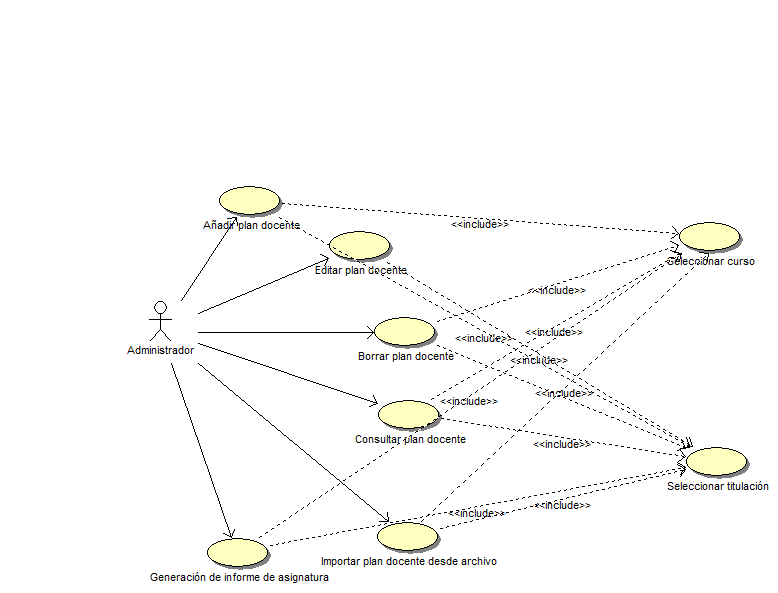
\includegraphics[scale=0.5]{./gestionplanificacion.png}
  \end{center}
\caption{Diagrama de casos de uso de la gestión de la planificación docente}
\end{figure}
\subsubsection*{Caso de uso: Añadir plan docente}
\begin{itemize}
\item{\bf Descripción:} Se añaden los detalles del plan docente para una asignatura en un curso determinado.
\item{\bf Actores:} Subdirector.
\item{\bf Precondiciones:} Ninguna.
\item{\bf Postcondiciones:} El plan docente queda registrado en el sistema, asociado a una asignatura y un curso determinado.
\item{\bf Escenario principal:}
	\begin{enumerate}
	\item Se realiza el caso de uso {\em \hyperref[select_asignatura]{Seleccionar asignatura}}.
	\item Se realiza el caso de uso {\em \hyperref[select_curso]{Seleccionar curso}}.
	\item El sistema comprueba que no exista ya un plan docente asociado a ese curso.
	\item El usuario introduce los datos del plan docente.
	\item El sistema comprueba que los datos cumplen el formato requerido.
	\item El sistema guarda la carga de trabajo y muestra un mensaje confirmándolo.
	\end{enumerate}
\item{\bf Escenarios alternativos:}
	\begin{itemize}
	\item[3.a.] Ya existe una carga de trabajo establecida para el curso seleccionado.
		\begin{enumerate}
		\item El sistema indica el error y el caso de uso vuelve al paso anterior.
		\end{enumerate}
	\item[4.a.] El usuario indica que quiere tomar los datos de otra carga de un curso anterior.
		\begin{enumerate}
		\item Se realiza el caso de uso {\em \hyperref[duplicar_carga]{Duplicar carga de trabajo}}
		\end{enumerate}
	\item[5.a.] Alguno de los datos introducidos no cumple el formato correcto.
		\begin{enumerate}
		\item El sistema indica el error y se vuelve al paso anterior.
		\end{enumerate}
	\item[5.b.] Alguno de los campos obligatorios no ha sido rellenado.
		\begin{enumerate}
		\item El sistema indica el error y se vuelve al paso anterior.
		\end{enumerate}	
	\item[*a.] En cualquier momento el administrador decide cancelar el proceso.
		\begin{enumerate}
		\item El caso de uso se termina.
		\end{enumerate}
	\end{itemize}
\end{itemize}



\subsubsection*{Caso de uso: Editar plan docente}
\begin{itemize}
\item{\bf Descripción:} Se edita una carga de trabajo existente para un curso determinado.
\item{\bf Actores:} Subdirector.
\item{\bf Precondiciones:} Ninguna.
\item{\bf Postcondiciones:} La carga de trabajo queda modificada en el sistema.
\item{\bf Pasos:}
	\begin{enumerate}
	\item Se realiza el caso de uso {\em \hyperref[select_asignatura]{Seleccionar asignatura}}.
	\item Se realiza el caso de uso {\em \hyperref[select_curso]{Seleccionar curso}}.
	\item El sistema comprueba que exista una carga asociada a ese curso.
	\item El sistema muestra los datos de la carga en un formato editable.
	\item El usuario modifica los datos.
	\item El sistema comprueba que los datos cumplen el formato requerido.
	\item El sistema guarda los cambios y muestra un mensaje confirmándolo.
	\end{enumerate}
\item{\bf Escenarios alternativos:}
	\begin{itemize}
	\item[3.a.] No existe una carga de trabajo establecida para el curso seleccionado.
		\begin{enumerate}
		\item El sistema indica el error y el caso de uso vuelve al paso anterior.
		\end{enumerate}
	\item[5.a.] Alguno de los datos introducidos no cumple el formato correcto.
		\begin{enumerate}
		\item El sistema indica el error y se vuelve al paso anterior.
		\end{enumerate}
	\item[5.b.] Alguno de los campos obligatorios no ha sido rellenado.
		\begin{enumerate}
		\item El sistema indica el error y se vuelve al paso anterior.
		\end{enumerate}	
	\item[*a.] En cualquier momento el administrador decide cancelar el proceso.
		\begin{enumerate}
		\item El caso de uso se termina.
		\end{enumerate}
	\end{itemize}
\end{itemize}



\subsubsection*{Caso de uso: Borrar plan docente}
\begin{itemize}
\item{\bf Descripción:} Se borra una carga de trabajo existente en el sistema asociada a un curso.
\item{\bf Actores:} Subdirector.
\item{\bf Precondiciones:} Ninguna.
\item{\bf Postcondiciones:} La carga de trabajo asociada a la asignatura y curso seleccionados queda. eliminada del sistema.
\item{\bf Escenario principal:}
	\begin{enumerate}
	\item Se realiza el caso de uso {\em \hyperref[select_asignatura]{Seleccionar asignatura}}
	\item Se realiza el caso de uso {\em \hyperref[select_curso]{Seleccionar curso}}.
	\item El sistema comprueba que exista una carga asociada a ese curso.
	\item El sistema muestra un diálogo de confirmación.
	\item El usuario confirma que desea borrar la carga.
	\item El sistema muestra un mensaje confirmando la eliminación y borra la carga.
	\end{enumerate}
\item{\bf Escenarios alternativos:}
	\begin{itemize}
	\item[3.a.] No existe una carga de trabajo establecida para el curso seleccionado.
	  \begin{enumerate}
	  \item El sistema indica el error y el caso de uso vuelve al paso anterior.
	  \end{enumerate}
	\item[5.a.] El administrador selecciona que no desea eliminar la carga.
		\begin{enumerate}
		\item El caso de uso se reinicia.
		\end{enumerate}
	\item[*a.] En cualquier momento el administrador decide cancelar la eliminación.
		\begin{enumerate}
		\item El caso de uso se termina.
		\end{enumerate}
	\end{itemize}
\end{itemize}



\subsubsection*{Caso de uso: Consultar plan docente}
\begin{itemize}
\item{\bf Descripción:} Se consulta la carga de trabajo de una asignatura para un curso determinado.
\item{\bf Actores:} Usuario.
\item{\bf Precondiciones:} Ninguna.
\item{\bf Postcondiciones:} Se muestran los datos al usuario por pantalla.
\item{\bf Escenario principal:}
	\begin{enumerate}
	\item Se realiza el caso de uso {\em \hyperref[select_asignatura]{Seleccionar asignatura}}
	\item Se realiza el caso de uso {\em \hyperref[select_curso]{Seleccionar curso}}.
	\item El sistema comprueba que exista una carga asociada a ese curso.
	\item La carga existe y es mostrada al usuario.
	\end{enumerate}
\item{\bf Escenarios alternativos:}
	\begin{itemize}
	\item[3.a.]No existe ninguna carga asociada a ese curso.
		\begin{enumerate}
		\item El sistema muestra un mensaje informando del error y vuelve al paso anterior.
		\end{enumerate}
	\item[*a.]En cualquier momento el usuario decide cancelar el proceso.
		\begin{enumerate}
		\item El caso de uso se cancela.
		\end{enumerate}		
	\end{itemize}
\end{itemize}




\subsubsection*{Caso de uso: Importar plan docente desde archivo}
\begin{itemize}
\item{\bf Descripción:} Caso de uso para importar planes docentes de forma masiva desde un archivo csv con un formato concreto.
\item{\bf Actores:} Administrador
\item{\bf Precondiciones:} El archivo tiene el formato correcto.
\item{\bf Postcondiciones:} Se crean los planes docentes indicados en el archivo.
\item{\bf Escenario principal:}
	\begin{enumerate}
	\item El administrador selecciona el archivo.
	\item El sistema comprueba que cada línea tenga el formato correcto.
	\item El sistema crea un plan docente por cada línea con los datos indicados en el archivo.
	\end{enumerate}
\item{\bf Escenarios alternativos:}
	\begin{itemize}
		\item[2.a.] Alguna línea no cumple el formato
		\begin{enumerate}
			\item El sistema indica el error y el caso de uso finaliza.
		\end{enumerate}
		\item[2.b.] Ya existe un plan docente creado para la asignatura indicada y para ese curso.
		\begin{enumerate}
			\item El sistema lo indica y el caso de uso finaliza.
		\end{enumerate}
	\end{itemize}
\end{itemize}


\subsubsection*{Caso de uso: Generación de informe de asignatura}
\begin{itemize}
\item{\bf Descripción:} Caso de uso para generar un informe de las horas asignadas a una asignatura.
\item{\bf Actores:} Administrador
\item{\bf Precondiciones:} La asignatura tiene un plan docente creado y asignadas horas en los horarios.
\item{\bf Postcondiciones:} Se genera un informe en pdf permitiendo su descarga.
\item{\bf Escenario principal:}
	\begin{enumerate}
	\item Se realiza el caso de uso {\em \hyperref[select_curso]{Seleccionar curso}}.
	\item Se realiza el caso de uso {\em \hyperref[select_asignatura]{Seleccionar asignatura}}.
	\item El sistema comprueba el plan docente de la asignatura y las asignaciones en los horarios.
	\item El sistema muestra un desglose de las horas de cada actividad de la asignatura y de cada semana teniendo en cuenta los eventos del calendario, permitiendo la descarga del archivo.
	\end{enumerate}
\item{\bf Escenarios alternativos:}
	\begin{itemize}
		\item[*.a.] En cualquier momento se decide parar el proceso.
		\begin{enumerate}
			\item El caso de uso finaliza.
		\end{enumerate}
		\item[3.a] La asignatura no tiene un plan docente asignado.
		\begin{enumerate}
			\item El caso de uso finaliza.
		\end{enumerate}
	\end{itemize}
\end{itemize}

\subsubsection{Gestión del calendario}
\begin{figure}[H] 
  \label{gestion-calendario} 
	\begin{center}
    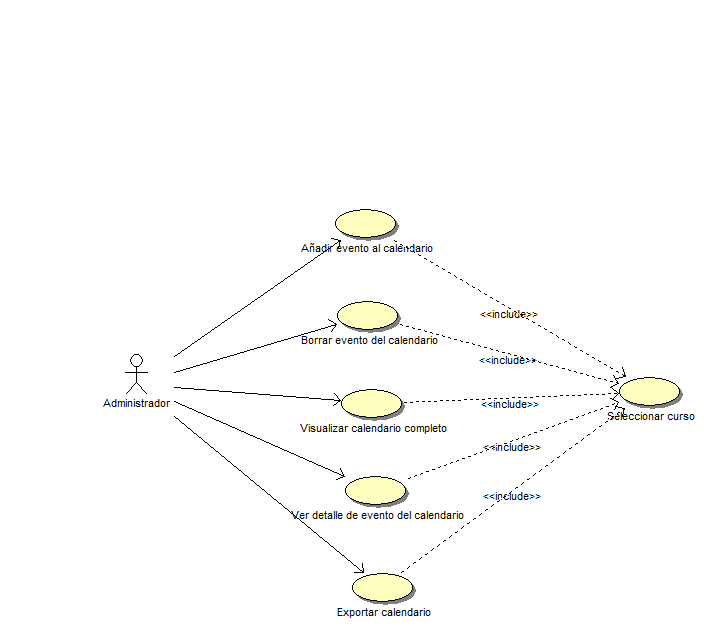
\includegraphics[scale=0.5]{./gestioncalendario.png}
  \end{center}
\caption{Diagrama de casos de uso de la gestión del calendario}
\end{figure}


\subsubsection*{Caso de uso: Añadir evento al calendario}
\begin{itemize}
\item{\bf Descripción:} Añade un evento de fechas al calendario, que puede ser una festividad o un período de vacaciones.
\item{\bf Actores:} Subdirector.
\item{\bf Precondiciones:} Ninguna.
\item{\bf Postcondiciones:} El evento queda registrado para el calendario de un curso concreto.
\item{\bf Escenario principal:}
	\begin{enumerate}
	\item Se realiza el caso de uso {\em \hyperref[select_curso]{Seleccionar curso}}.
	\item El subdirector introduce los datos correspondientes al evento, que serían, el nombre del evento, el tipo de evento, si es una fecha concreta o un rango de ellas, y su fecha de inicio y finalización.
	\item El sistema comprueba que los datos son correctos y que no se solapen con otros eventos.
	\item El sistema indica que todo es correcto y muestra un mensaje confirmando el éxito de la operación.
	\end{enumerate}
\item{\bf Escenarios alternativos:}
	\begin{itemize}
		\item[3.a.] Alguno de los datos tiene un formato incorrecto o algún campo está en blanco.
		\begin{enumerate}
			\item El sistema lo indica y vuelve al paso anterior.
		\end{enumerate}
		\item[3.b.] Las fechas del evento se solapan con algún otro evento o fecha del curso.
		\begin{enumerate}
			\item El sistema lo indica y vuelve al paso anterior.
		\end{enumerate}
		\item[*a.] En cualquier momento el usuario decide cancelar el proceso.
		\begin{enumerate}
		\item El caso de uso finaliza.
		\end{enumerate}
	\end{itemize}
\end{itemize}



\subsubsection*{Caso de uso: Borrar evento del calendario}
\begin{itemize}
\item{\bf Descripción:} El usuario selecciona alguno de los eventos del calendario para eliminarlo y este queda eliminado del sistema.
\item{\bf Actores:} Subdirector.
\item{\bf Precondiciones:} Ninguna.
\item{\bf Postcondiciones:} El evento queda eliminado del calendario del curso concreto.
\item{\bf Escenario principal:}
	\begin{enumerate}
	\item Se realiza el caso de uso {\em \hyperref[select_curso]{Seleccionar curso}}.
	\item El sistema muestra un listado de fechas de eventos.
	\item El subdirector selecciona la fecha que desea eliminar.
	\item El sistema muestra un mensaje confirmando que el evento ha sido eliminado.
	\end{enumerate}
\item{\bf Escenarios alternativos:}
	\begin{itemize}
		\item[2.a.] No hay ningún evento registrado en el calendario de ese curso.
		\begin{enumerate}
			\item El sistema lo indica y el caso de uso finaliza.
		\end{enumerate}
		\item[*a.] En cualquier momento el subdirector decide cancelar el proceso.
		\begin{enumerate}
		\item El caso de uso finaliza sin eliminar el evento.
		\end{enumerate}
	\end{itemize}
\end{itemize}



\subsubsection*{Caso de uso: Visualizar calendario completo}
\begin{itemize}
\item{\bf Descripción:} Se muestra un calendario completo con las fechas marcadas.
\item{\bf Actores:} Usuario.
\item{\bf Precondiciones:} Ninguna.
\item{\bf Postcondiciones:} Se muestra el calendario por pantalla.
\item{\bf Escenario principal:}
	\begin{enumerate}
	\item Se realiza el caso de uso {\em \hyperref[select_curso]{Seleccionar curso}}.
	\item El sistema muestra un calendario con las fechas de los eventos marcadas.
	\end{enumerate}
\item{\bf Escenarios alternativos:}
\end{itemize}


\subsubsection*{Caso de uso: Ver detalle de evento del calendario}
\begin{itemize}
\item{\bf Descripción:} Se muestran los datos detallados de un evento del calendario
\item{\bf Actores:} Usuario
\item{\bf Precondiciones:} Hay eventos registrados en el sistema
\item{\bf Postcondiciones:} Se muestran los datos.
\item{\bf Escenario principal:}
	\begin{enumerate}
	\item Se realiza el caso de uso {\em \hyperref[select_curso]{Seleccionar curso}}.
	\item El sistema muestra el calendario para el curso actual con los eventos creados sobre él.
	\item El usuario selecciona un evento
	\item El sistema muestra los datos del evento, título, razón, etc.
	\end{enumerate}
\item{\bf Escenarios alternativos:}
\end{itemize}




\subsubsection*{Caso de uso: Exportar calendario}
\begin{itemize}
\item{\bf Descripción:} Caso de uso para exportar el calendario de un curso a un formato externo como csv o una hoja de cálculo.
\item{\bf Actores:} Administrador.
\item{\bf Precondiciones:} El curso existe y tiene eventos creados.
\item{\bf Postcondiciones:} Se exporta un archivo con un formato adecuado.
\item{\bf Escenario principal:}
	\begin{enumerate}
	\item Se realiza el caso de uso {\em \hyperref[select_curso]{Seleccionar curso}}.
	\item Se muestra y permite descarga del archivo exportado.
	\end{enumerate}
\item{\bf Escenarios alternativos:}
	\begin{itemize}
		\item[*.a.] En cualquier momento el administrador decide cancelar el proceso.
		\begin{enumerate}
			\item Se finaliza el caso de uso.
		\end{enumerate}
	\end{itemize}
\end{itemize}


\subsubsection{Gestión de horarios}
\begin{figure}[H] 
  \label{gestion-horarios} 
	\begin{center}
    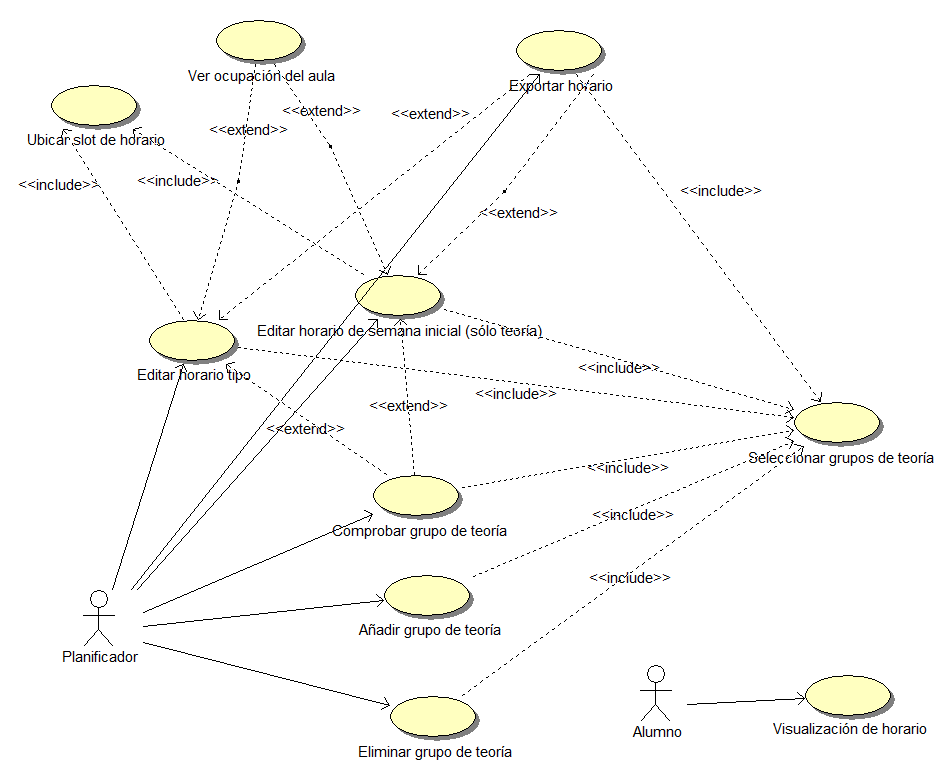
\includegraphics[scale=0.5]{./gestionhorarios.png}
  \end{center}
\caption{Diagrama de casos de uso de la gestión de titulaciones}
\end{figure}

\subsubsection*{Caso de uso: Seleccionar grupos de teoría}
\label{select_grupo}
\begin{itemize}
\item{\bf Descripción:} Se muestran los grupos de teoría de una titulación. Este caso de uso es incluido por más casos de uso.
\item{\bf Actores:} Administrador
\item{\bf Precondiciones:} Hay titulaciones y cursos creados.
\item{\bf Postcondiciones:} Se muestra la información
\item{\bf Escenario principal:}
	\begin{enumerate}
	\item Se realiza el caso de uso {\em \hyperref[select_curso]{Seleccionar curso}}.
	\item Se realiza el caso de uso {\em \hyperref[select_titulacion]{Seleccionar titulación}}.
	\item El sistema muestra un listado con los cursos de la titulación y el número de grupos de cada curso.
	\item El administrador selecciona el grupo deseado.
	\end{enumerate}
\item{\bf Escenarios alternativos:}
\end{itemize}



\subsubsection*{Caso de uso: Ubicar slot de horario}
\label{guardar_slot}
\begin{itemize}
\item{\bf Descripción:} Caso de uso abstracto que es incluído por otros casos de uso. Se utiliza para ubicar en un horario un slot de una actividad de una asignatura.
\item{\bf Actores:} Administrador
\item{\bf Precondiciones:} La asignatura existe y tiene asignadas horas en el plan docente para esa actividad.
\item{\bf Postcondiciones:} El slot de la actividad queda guardado en el horario.
\item{\bf Escenario principal:}
	\begin{enumerate}
	\item El administrador selecciona una asignatura y su actividad
	\item El sistema comprueba que tenga asignadas horas en el plan docente
	\item El administrador selecciona el aula en la que se guardará el slot
	\item El administrador selecciona el lugar que ocupará en el horario
	\item El sistema comprueba que el aula no esté ocupada en ese momento y que si el slot es de teoría que no se solape con otros slots.
	\item El sistema guarda el slot en el horario.
	\end{enumerate}
\item{\bf Escenarios alternativos:}
	\begin{itemize}
		\item[2.a.] La asignatura no tiene horas asignadas para esa actividad.
		\begin{enumerate}
			\item El sistema lo indica y se vuelve al paso anterior.
		\end{enumerate}
		\item[5.a.] El aula está ocupada en ese horario.
		\begin{enumerate}
			\item El sistema lo indica y se vuelve al paso 3.
		\end{enumerate}
		\item[5.b.] El slot es de teoría y se solapa con otros slots.
		\begin{enumerate}
			\item El sistema lo indica y se vuelve al paso anterior.
		\end{enumerate}
	\end{itemize}
\end{itemize}



\subsubsection*{Caso de uso: Editar horario tipo}
\begin{itemize}
\item{\bf Descripción:} Se muestra el horario de un grupo de teoría en un formato editable.
\item{\bf Actores:} Administrador
\item{\bf Precondiciones:} Hay algún grupo creado para la titulación, semestre, curso y año académico.
\item{\bf Postcondiciones:} Se muestran las asignaturas disponibles, permitiendo su edición. Se muestran tanto los slots de teoría como los de las demás actividades
\item{\bf Escenario principal:}
	\begin{enumerate}
	\item Se realiza el caso de uso {\em \hyperref[select_grupo]{Seleccionar grupos de teoría}}.
	\item El administrador selecciona el curso y semestre deseado para editar su horario tipo.
	\item El sistema comprueba que exista el grupo y se que no exista un horario ya empezado.
	\item Se realiza el caso de uso {\em \hyperref[guardar_slot]{Ubicar slot de horario}}.
	\item El administrador realiza el paso anterior las veces que sean necesarias hasta completar el horario.
	\end{enumerate}
\item{\bf Escenarios alternativos:}
	\begin{itemize}
		\item[*.a.] En cualquier momento el administrador decide parar el proceso.
		\begin{enumerate}
			\item El sistema guarda los cambios hechos hasta ahora y el caso de uso finaliza.
		\end{enumerate}
		\item[2.a] No ha sido creado ningún grupo para ese curso.
		\begin{enumerate}
			\item El sistema indica el error y finaliza el caso de uso.
		\end{enumerate}
		\item[3.a] Ya hay un horario empezado para ese grupo y semestre
		\begin{enumerate}
			\item El sistema muestra el horario ya empezado ubicando los slots donde estaban en el antiguo horario y el caso de uso continua.
		\end{enumerate}
	\end{itemize}
\end{itemize}



\subsubsection*{Caso de uso: Editar horario de semana inicial (sólo teoría)}
\begin{itemize}
\item{\bf Descripción:} Se muestra para su edición el horario de un grupo de teoría en una semana en la que sólo se imparte teoría
\item{\bf Actores:} Administrador
\item{\bf Precondiciones:} Ya ha sido creado el grupo y editado el horario tipo correspondiente
\item{\bf Postcondiciones:} Se muestra el horario con los slots de teoría del horario tipo ubicados en su sitio, salvo los que no sean posible por no ser día lectivo
\item{\bf Escenario principal:}
	\begin{enumerate}
	\item Se realiza el caso de uso {\em \hyperref[select_grupo]{Seleccionar grupo de teoría}}.
	\item El administrador selecciona el curso y semestre además de la semana que se editará.
	\item El sistema comprueba que exista el grupo y se que no exista un horario ya empezado.
	\item El sistema muestra los slots de teoría del horario tipo correspondiente, sacando del horario los que no sean posibles ubicar automáticamente por que el día sea no lectivo.
	\item Se realiza el caso de uso {\em \hyperref[guardar_slot]{Ubicar slot de horario}}.
	\item Se realiza el paso anterior las veces que se consideren necesarias hasta completar el horario.
	\end{enumerate}
\item{\bf Escenarios alternativos:}
	\begin{itemize}
		\item[*.a.] En cualquier momento el administrador decide parar el proceso.
		\begin{enumerate}
			\item El sistema guarda los cambios hechos hasta ahora y el caso de uso finaliza.
		\end{enumerate}
		\item[2.a] No ha sido creado ningún grupo para ese curso.
		\begin{enumerate}
			\item El sistema indica el error y finaliza el caso de uso.
		\end{enumerate}
		\item[3.a] Ya hay un horario empezado para ese grupo, semestre y semana
		\begin{enumerate}
			\item El sistema muestra el horario ya empezado ubicando los slots donde estaban en el antiguo horario y el caso de uso continua.
		\end{enumerate}
	\end{itemize}
\end{itemize}



\subsubsection*{Caso de uso: Añadir grupo de teoría}
\begin{itemize}
\item{\bf Descripción:} Se añade un grupo de teoría a un curso de una titulación para poder editar más adelante su horario
\item{\bf Actores:} Administrador
\item{\bf Precondiciones:} La titulación existe y tiene asignaturas con planes docentes creados para el curso actual.
\item{\bf Postcondiciones:} El grupo se añade al curso correspondiente.
\item{\bf Escenario principal:}
	\begin{enumerate}
	\item Se realiza el caso de uso {\em \hyperref[select_grupo]{Seleccionar grupo de teoría}}.
	\item El administrador selecciona el curso de la titulación al que se va a añadir el grupo.
	\item El sistema comprueba que no se haya sobrepasado el número de grupos indicado en el plan docente y guarda el grupo.
	\end{enumerate}
\item{\bf Escenarios alternativos:}
	\begin{itemize}
		\item[2.a.] Se han sobrepasado el número de grupos indicado en el plan docente.
		\begin{enumerate}
			\item El sistema advierte del problema pero el caso de uso continúa.
		\end{enumerate}
	\end{itemize}
\end{itemize}



\subsubsection*{Caso de uso: Eliminar grupo de teoría}
\begin{itemize}
\item{\bf Descripción:} Se elimina un grupo de teoría de un curso de una titulación
\item{\bf Actores:} Administrador
\item{\bf Precondiciones:} Hay grupos creados para la titulación y curso.
\item{\bf Postcondiciones:} Se elimina el grupo así como toda su información asociada (horarios, informes, etc).
\item{\bf Escenario principal:}
	\begin{enumerate}
	\item Se realiza el caso de uso {\em \hyperref[select_grupo]{Seleccionar grupo de teoría}}.
	\item El administrador selecciona el curso de la titulación al que se va a eliminar el grupo.
	\item El sistema pide confirmación de la eliminación.
	\item El administrador confirma que desea eliminar el grupo.
	\item Queda borrado el grupo y toda la información asociada y el sistema lo indica.
	\end{enumerate}
\item{\bf Escenarios alternativos:}
	\begin{itemize}
		\item[4.a.] El administrador cancela el proceso.
		\begin{enumerate}
			\item El caso de uso finaliza.
		\end{enumerate}
	\end{itemize}
\end{itemize}



\subsubsection*{Caso de uso: Exportar horario}
\begin{itemize}
\item{\bf Descripción:} Caso de uso para exportar un horario creado a un formato externo como csv o una hoja de cálculo.
\item{\bf Actores:} Administrador.
\item{\bf Precondiciones:} Existe un grupo creado y está creado el horario.
\item{\bf Postcondiciones:} Se exporta un archivo con un formato adecuado.
\item{\bf Escenario principal:}
	\begin{enumerate}
	\item Se realiza el caso de uso {\em \hyperref[select_grupo]{Seleccionar grupo de teoría}}.
	\item El administrador selecciona la semana, semestre y curso.
	\item El sistema busca el horario elegido.
	\item Se muestra y permite descarga del archivo exportado.
	\end{enumerate}
\item{\bf Escenarios alternativos:}
	\begin{itemize}
		\item[*.a.] En cualquier momento el administrador decide cancelar el proceso.
		\begin{enumerate}
			\item El caso de uso finaliza.
		\end{enumerate}
		\item[3.a.] No existe un horario creado para los datos elegidos.
		\begin{enumerate}
			\item El sistema lo indica y se vuelve al paso anterior.
		\end{enumerate}
	\end{itemize}
\end{itemize}


\subsubsection*{Caso de uso: Comprobar grupo de teoría}
\begin{itemize}
\item{\bf Descripción:} Caso de uso para comprobar que el número de horas introducidas en los horarios de un grupo coincide con lo indicado en el plan docente de cada asignatura.
\item{\bf Actores:} Administrador.
\item{\bf Precondiciones:} El grupo existe y tiene horarios creados.
\item{\bf Postcondiciones:} Se muestra la comprobación indicando si faltan o sobran horas en las asignaturas y actividades.
\item{\bf Escenario principal:}
	\begin{enumerate}
	\item Se realiza el caso de uso {\em \hyperref[select_grupo]{Seleccionar grupo de teoría}}.
	\item El sistema muestra el cálculo de horas de un grupo mediante los horarios de esa semana, teniendo en cuenta los eventos asignados en el calendario e indica dónde faltan horas por asignar para que sea solucionado.
	\end{enumerate}
\item{\bf Escenarios alternativos:}
	\begin{itemize}
		\item[*.a.] En cualquier momento se decide parar el proceso.
		\begin{enumerate}
			\item El caso de uso finaliza.
		\end{enumerate}
	\end{itemize}
\end{itemize}



\subsubsection{Gestión de aulas}
\begin{figure}[H] 
  \label{gestion-aulas} 
	\begin{center}
    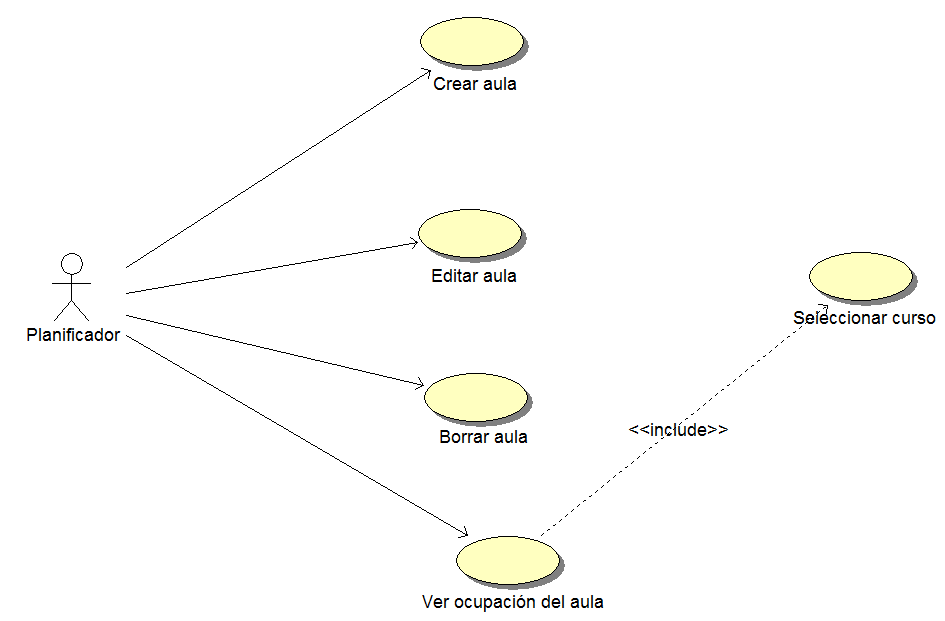
\includegraphics[scale=0.5]{./gestionaulas.png}
  \end{center}
\caption{Diagrama de casos de uso de la gestión de aulas}
\end{figure}
\subsubsection*{Caso de uso: Crear aula}
\begin{itemize}
\item{\bf Descripción:} Caso de uso para crear un aula a la que asignar slots de horario
\item{\bf Actores:} Administrador
\item{\bf Precondiciones:} Ninguna
\item{\bf Postcondiciones:} El aula queda creada
\item{\bf Escenario principal:}
	\begin{enumerate}
	\item El administrador introduce los datos del aula: nombre y actividades para las que sirve
	\item El sistema comprueba que no exista ningún aula con ese nombre y el aula queda creada.
	\end{enumerate}
\item{\bf Escenarios alternativos:}
	\begin{itemize}
		\item[*.a.] En cualquier momento el administrador decide cancelar el proceso.
		\begin{enumerate}
			\item El caso de uso finaliza.
		\end{enumerate}
		\item[2.a.] Ya existe un aula con ese nombre.
		\begin{enumerate}
			\item El sistema lo indica y se vuelve al paso anterior.
		\end{enumerate}
	\end{itemize}
\end{itemize}



\subsubsection*{Caso de uso: Editar aula}
\begin{itemize}
\item{\bf Descripción:} Caso de uso para editar los datos de un aula ya creada
\item{\bf Actores:} Administrador
\item{\bf Precondiciones:} El aula existe.
\item{\bf Postcondiciones:} El aula queda guardada con los nuevos datos.
\item{\bf Escenario principal:}
	\begin{enumerate}
	\item El sistema muestra los datos actuales del aula permitiendo su edición
	\item El administrador edita el nombre y añade o elimina actividades.
	\item El sistema valida que el nuevo nombre no exista y guarda los datos
	\end{enumerate}
\item{\bf Escenarios alternativos:}
	\begin{itemize}
		\item[*.a.] En cualquier momento el administrador decide cancelar el proceso
		\begin{enumerate}
			\item El caso de uso finaliza.
		\end{enumerate}
		\item[3.a.] Ya existe un aula con ese nombre
		\begin{enumerate}
			\item El sistema lo indica y se vuelve al paso anterior
		\end{enumerate}
	\end{itemize}
\end{itemize}



\subsubsection*{Caso de uso: Eliminar aula}
\begin{itemize}
\item{\bf Descripción:} Caso de uso para eliminar un aula del sistema.
\item{\bf Actores:} Administrador.
\item{\bf Precondiciones:} El aula existe en el sistema.
\item{\bf Postcondiciones:} El aula queda eliminada del sistema y todas las referencias a ésta quedan borradas.
\item{\bf Escenario principal:}
	\begin{enumerate}
	\item Se selecciona el aula a eliminar
	\item El sistema pide confirmación
	\item El administrador confirma la eliminación
	\item El sistema elimina el aula y borra todas las referencias a ésta.
	\end{enumerate}
\item{\bf Escenarios alternativos:}
	\begin{itemize}
		\item[3.a.] El administrador decide que no desea eliminar el aula.
		\begin{enumerate}
			\item El caso de uso finaliza
		\end{enumerate}
	\end{itemize}
\end{itemize}



\subsubsection*{Caso de uso: Ver ocupación de aula}
\begin{itemize}
\item{\bf Descripción:} Caso de uso para ver la ocupación actual de un aula según los horarios creados para el curso actual.
\item{\bf Actores:} Administrador.
\item{\bf Precondiciones:} El aula existe en el sistema.
\item{\bf Postcondiciones:} Se muestran todos los slots que están asignados a ese aula junto con su horario.
\item{\bf Escenario principal:}
	\begin{enumerate}
	\item El administrador selecciona el aula para la que desea ver la ocupación.
	\item El administrador selecciona el semestre y la semana para el que desea ver la ocupación.
	\item El sistema muestra la ocupación actual.
	\end{enumerate}
\item{\bf Escenarios alternativos:}
	\begin{itemize}
		\item[*.a.] En cualquier momento el administrador decide cancelar el proceso.
		\begin{enumerate}
			\item El caso de uso finaliza.
		\end{enumerate}
	\end{itemize}
\end{itemize}

\section{Modelo conceptual de datos}

\subsection{Diagrama de clases conceptuales}

\begin{figure}[H] 
  \label{modelo-conceptual} 
	\begin{center}
    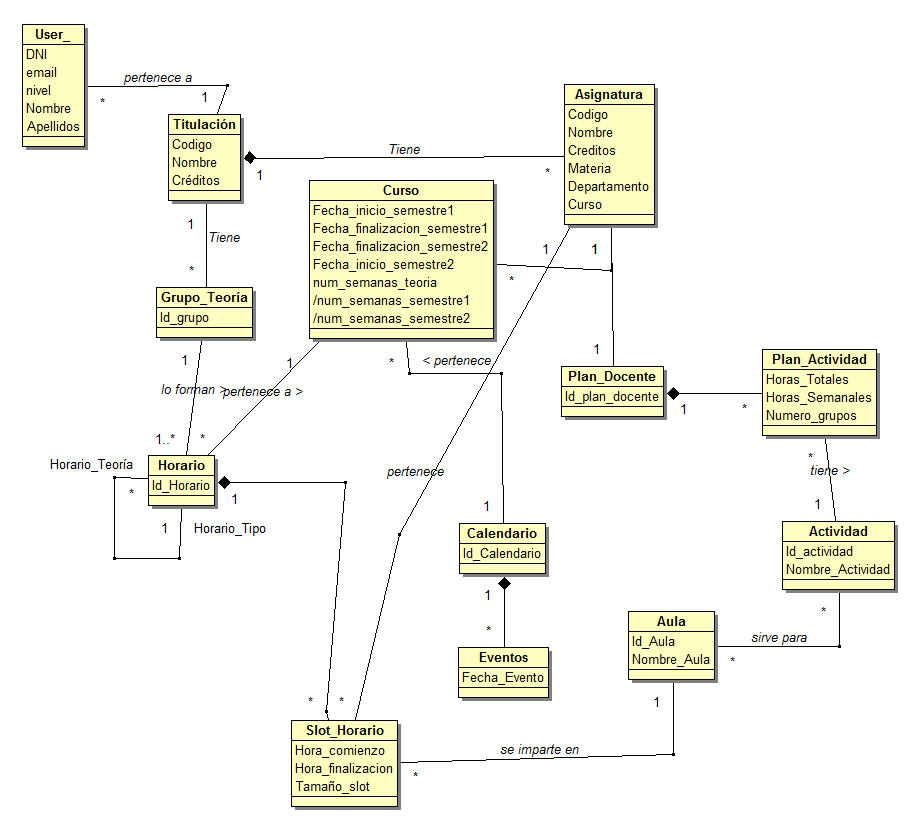
\includegraphics[scale=0.7]{./modeloconceptual.png}
  \end{center}
\caption{Diagrama del modelo conceptual de datos}
\end{figure}

\section{Modelo de comportamiento del sistema}

Para el modelo de comportamiento del sistema se mostrarán diferentes diagramas de secuencia del sistema. El diagrama define las interacciones entre actores y sistema, también se detallarán los contratos de las operaciones del sistema, para describir en detalle qué hace cada operación.
\paragraph{}
Al existir muchos casos de uso similares, sólo se detallarán los más relevantes de cada subsistema.

\subsection{Caso de uso: Registrar titulación}

\begin{figure}[H] 
  \label{comportamiento-reg-titulacion} 
	\begin{center}
    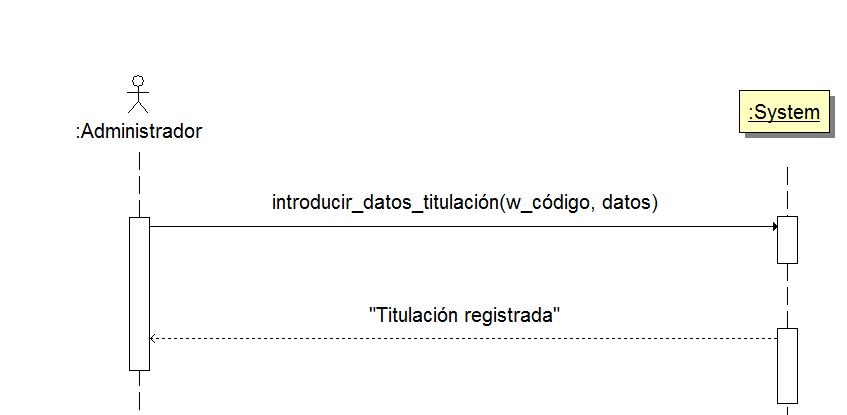
\includegraphics[scale=0.5]{./secuencia-reg-titulacion.png}
  \end{center}
\caption{Diagrama de secuencia del caso de uso Registrar titulación}
\end{figure}

\subsubsection{Contrato de la operación: introducir\_datos\_titulación}
\begin{itemize}
\item {\bf Responsabilidades:} Registrar una titulación en el sistema.
\item {\bf Referencias cruzadas:} Caso de uso {\em registrar titulación}, Caso de uso {\em editar titulación}.
\item {\bf Precondiciones:} No existe ninguna titulación con código = w\_código.
\item {\bf Postcondiciones:} Se crea una instancia T de Titulación. Se asignan w\_código y datos a T.
\end{itemize}

\subsection{Caso de uso: Registrar asignatura}

\begin{figure}[H] 
  \label{comportamiento-reg-asignatura} 
	\begin{center}
    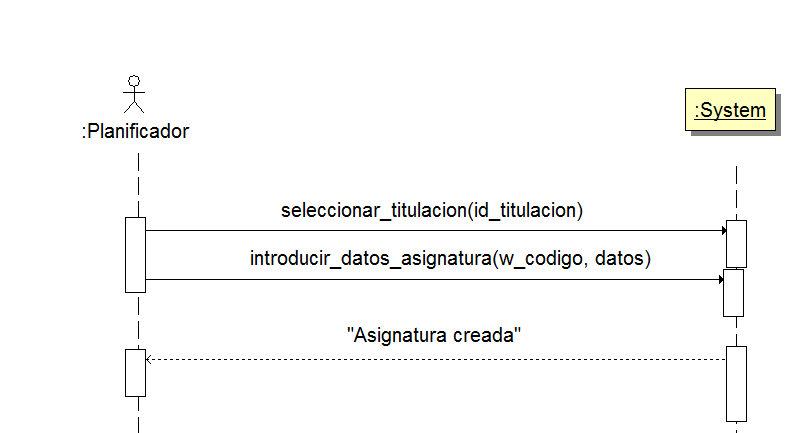
\includegraphics[scale=0.5]{./secuencia-reg-asignatura.png}
  \end{center}
\caption{Diagrama de secuencia del caso de uso Registrar asignatura}
\end{figure}

\subsubsection{Contrato de la operación: seleccionar\_titulacion}
\begin{itemize}
\item {\bf Responsabilidades:} Seleccionar una titulación para añadirle una asignatura.
\item {\bf Referencias cruzadas:} Caso de uso {\em registrar asignatura}, Caso de uso {\em editar asignatura}
\item {\bf Precondiciones:} Existe una titulación con t.id = id\_titulación.
\item {\bf Postcondiciones:} Se devuelve una instancia T de Titulación con T.id = id\_titulación.
\end{itemize}

\subsubsection{Contrato de la operación: introducir\_datos\_asignatura}
\begin{itemize}
\item {\bf Responsabilidades:} Registrar una asignatura y asociarla a una titulación.
\item {\bf Referencias cruzadas:} Caso de uso {\em registrar asignatura}, Caso de uso {\em editar asignatura}
\item {\bf Precondiciones:} No existe ninguna asignatura con código = w\_codigo.
\item {\bf Postcondiciones:} Se crea una instancia A de Asignatura. Se asigna A.codigo = w\_codigo y A.datos = datos.
\end{itemize}

\subsection{Caso de uso: Editar asignatura}
\begin{figure}[H] 
  \label{comportamiento-edit-asignatura} 
	\begin{center}
    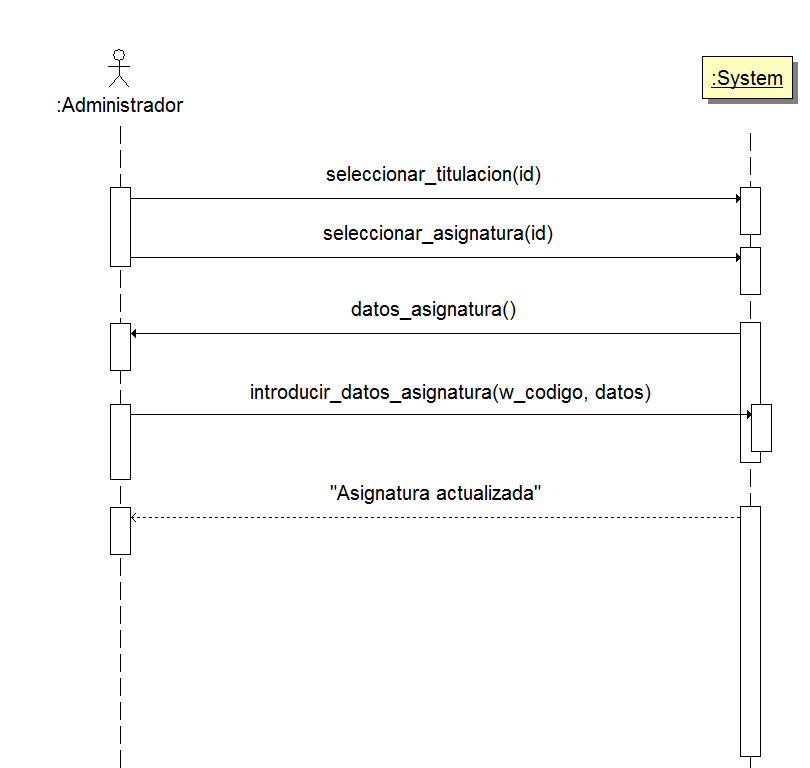
\includegraphics[scale=0.5]{./secuencia-edit-asignatura.png}
  \end{center}
\caption{Diagrama de secuencia del caso de uso Editar asignatura}
\end{figure}

\subsubsection{Contrato de la operación: seleccionar\_asignatura}
\begin{itemize}
\item {\bf Responsabilidades:} Devolver una instancia de Asignatura para poder editar sus datos.
\item {\bf Referencias cruzadas:} Caso de uso {\em editar asignatura}, Caso de uso {\em borrar asignatura}.
\item {\bf Precondiciones:} Debe existir una Asignatura registrada en el sistema con A.id = id\_asignatura.
\item {\bf Postcondiciones:} Se devuelve una instancia A de Asignatura con A.id = id\_asignatura.
\end{itemize}

\subsection{Caso de uso: Borrar asignatura}
\begin{figure}[H] 
  \label{comportamiento-borrar-asignatura} 
	\begin{center}
    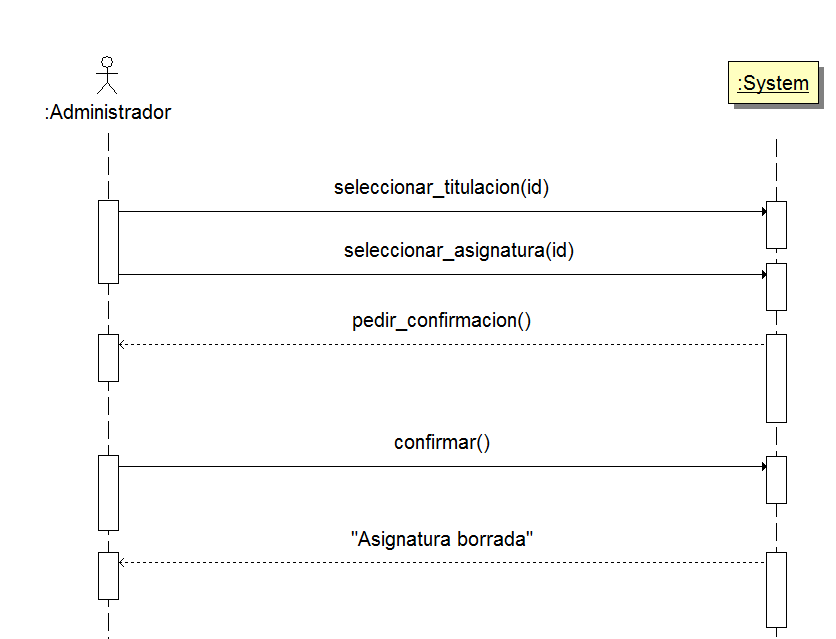
\includegraphics[scale=0.5]{./secuencia-borrar-asignatura.png}
  \end{center}
\caption{Diagrama de secuencia del caso de uso Borrar asignatura}
\end{figure}

\subsection{Caso de uso: Importar asignatura}
\begin{figure}[H] 
  \label{comportamiento-importar-asignatura} 
	\begin{center}
    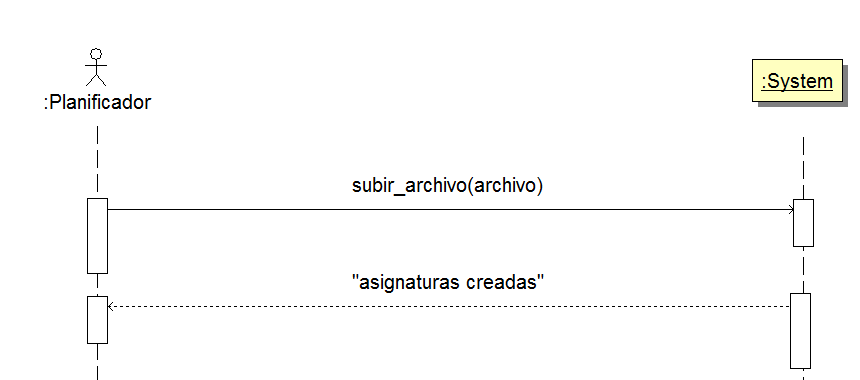
\includegraphics[scale=0.5]{./secuencia-importar-asignatura.png}
  \end{center}
\caption{Diagrama de secuencia del caso de uso Importar asignatura}
\end{figure}

\subsubsection{Contrato de la operación: subir\_archivo}
\begin{itemize}
\item {\bf Responsabilidades:} Crear asignaturas masivamente capturando la información de las líneas de un archivo.
\item {\bf Referencias cruzadas:} Caso de uso {\em importar asignatura}, Caso de uso {\em importar titulación}, Caso de uso {\em importar plan docente}.
\item {\bf Precondiciones:} Por cada línea del archivo, no existe una instancia de la clase a la que se pretende añadir información con la misma clave que aparece en la línea.
\item {\bf Postcondiciones:} Por cada línea se crea una instancia de la clase con id = id\_linea.
\end{itemize}

\subsection{Caso de uso: Crear plan docente}
\begin{figure}[H] 
  \label{comportamiento-crear-plandocente} 
	\begin{center}
    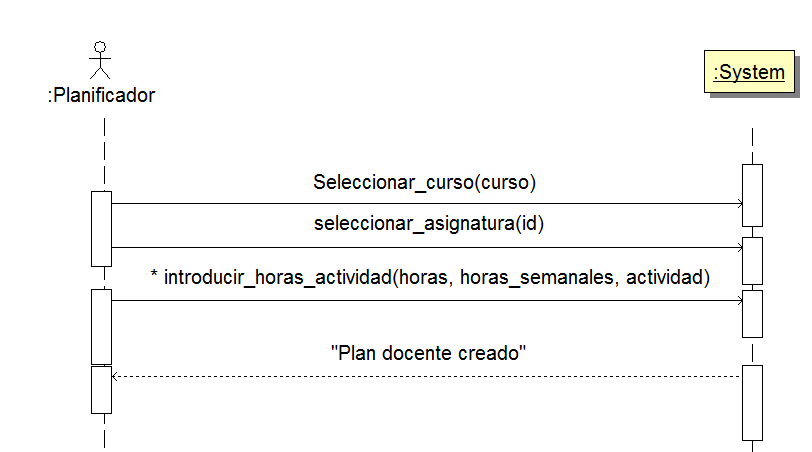
\includegraphics[scale=0.5]{./secuencia-crear-plandocente.png}
  \end{center}
\caption{Diagrama de secuencia del caso de uso Crear plan docente}
\end{figure}

\subsubsection{Contrato de la operación: introducir\_horas\_actividad}
\begin{itemize}
\item {\bf Responsabilidades:} Añadir la planificación docente de una actividad concreta al sistema.
\item {\bf Referencias cruzadas:} Caso de uso {\em crear plan docente}, Caso de uso {\em editar plan docente}
\item {\bf Precondiciones:} La actividad existe en el sistema.
\item {\bf Postcondiciones:} Se crea una instancia P de Plan\_Actividad con P.actividad = actividad, P.horas = horas y  P.horas\_semanales = horas\_semanales, además se asocia con la asignatura A.
\end{itemize}

\subsection{Caso de uso: Generar informe de asignatura}
\begin{figure}[H] 
  \label{comportamiento-generar-informe} 
	\begin{center}
    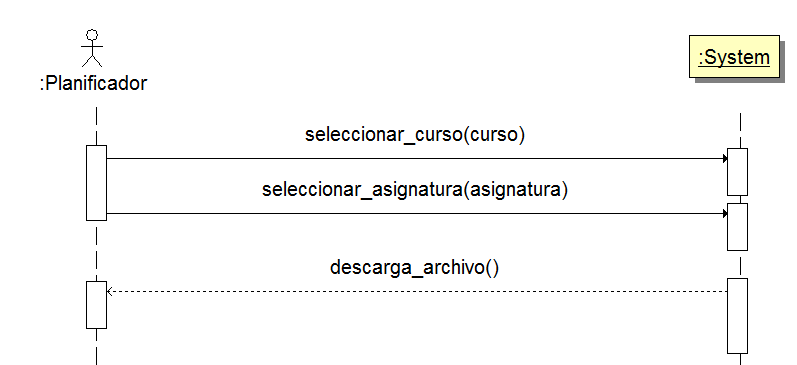
\includegraphics[scale=0.5]{./secuencia-gen-informe.png}
  \end{center}
\caption{Diagrama de secuencia del caso de uso Generar informe de asignatura}

\subsection{Caso de uso: Añadir evento al calendario}
\begin{figure}[H] 
  \label{comportamiento-anadir-evento} 
	\begin{center}
    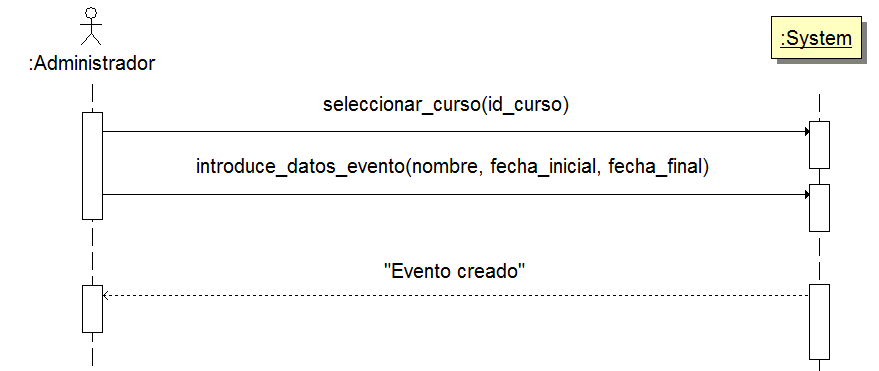
\includegraphics[scale=0.5]{./secuencia-crear-evento.png}
  \end{center}
\caption{Diagrama de secuencia del caso de uso Añadir evento al calendario}
\end{figure}
\end{figure}

\subsubsection{Contrato de la operación: seleccionar curso}
\begin{itemize}
\item {\bf Responsabilidades:} Seleccionar un curso para hacer operaciones con el o asociarlo con otras clases.
\item {\bf Referencias cruzadas:} Caso de uso {\em Añadir evento al calendario}.
\item {\bf Precondiciones:} Existe un curso C con C.id\_curso = id\_curso.
\item {\bf Postcondiciones:} Se devuelve una instancia C de curso.
\end{itemize}

\subsubsection{Contrato de la operación: introduce\_datos\_evento}
\begin{itemize}
\item {\bf Responsabilidades:} Crear un evento en el calendario del curso C.
\item {\bf Referencias cruzadas:} Caso de uso {\em Añadir evento al calendario}.
\item {\bf Precondiciones:} No existe ningún evento con fechas entre las introducidas.
\item {\bf Postcondiciones:} Se crea una instancia E de Evento con E.fecha\_inicial = fecha\_inicial, E.fecha\_final = fecha\_final y E.nombre = nombre y se asocia a C.
\end{itemize}

\subsection{Caso de uso: Exportar calendario}
\begin{figure}[H] 
  \label{comportamiento-exportar-calendario} 
	\begin{center}
    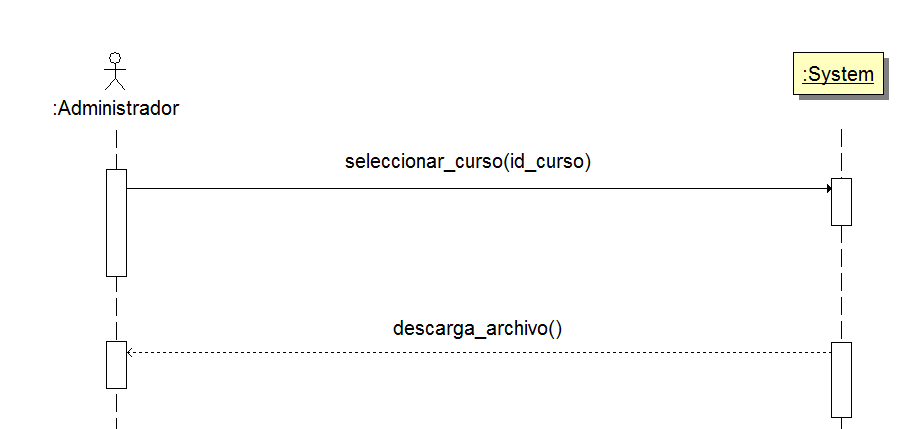
\includegraphics[scale=0.5]{./secuencia-exportar-calendario.png}
  \end{center}
\caption{Diagrama de secuencia del caso de uso Exportar calendario}
\end{figure}


\subsection{Caso de uso: Seleccionar grupos de teoría}
\begin{figure}[H] 
  \label{comportamiento-seleccionar-grupos} 
	\begin{center}
    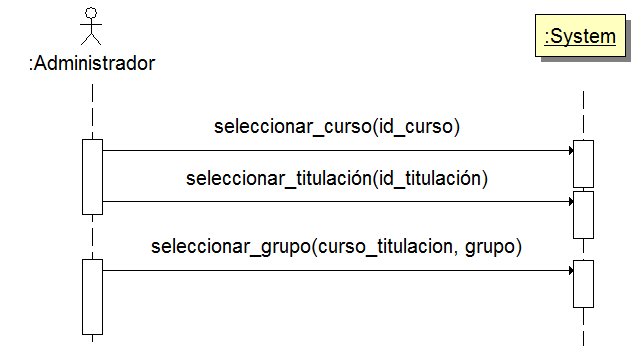
\includegraphics[scale=0.5]{./secuencia-seleccionar-grupo.png}
  \end{center}
\caption{Diagrama de secuencia del caso de uso Seleccionar grupos de teoría}
\end{figure}

\subsubsection{Contrato de la operación: seleccionar\_grupo}
\begin{itemize}
\item {\bf Responsabilidades:} Seleccionar un grupo de una titulación para hacer uso de él en otro caso de uso.
\item {\bf Referencias cruzadas:} Caso de uso {\em seleccionar grupos de teoría}
\item {\bf Precondiciones:} El curso indicado está dentro de los cursos de la titulación.
\\El grupo ha sido creado.
\item {\bf Postcondiciones:} Se devuelve una instancia G del Grupo.
\end{itemize}

\subsection{Caso de uso: Añadir grupo de teoría}
\begin{figure}[H] 
  \label{comportamiento-anadir-grupos} 
	\begin{center}
    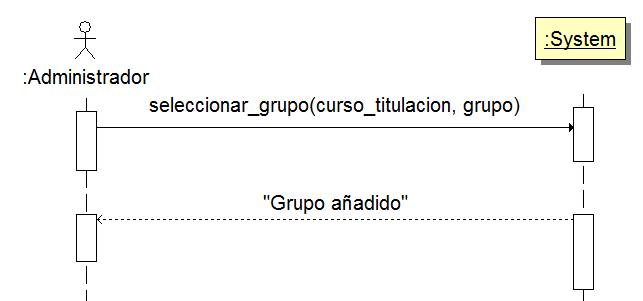
\includegraphics[scale=0.5]{./secuencia-anadir-grupo.png}
  \end{center}
\caption{Diagrama de secuencia del caso de uso Añadir grupo de teoría}
\end{figure}

\subsection{Caso de uso: Eliminar grupo de teoría}
\begin{figure}[H] 
  \label{comportamiento-borrar-grupos} 
	\begin{center}
    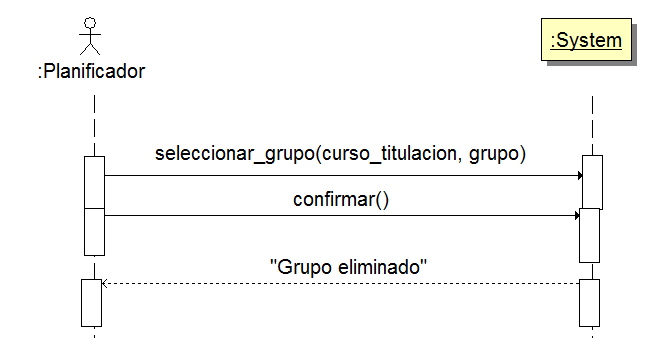
\includegraphics[scale=0.5]{./secuencia-borrar-grupo.png}
  \end{center}
\caption{Diagrama de secuencia del caso de uso Eliminar grupo de teoría}
\end{figure}

\subsection{Caso de uso: Ubicar slot de horario}
\begin{figure}[H] 
  \label{comportamiento-ubicar-slot} 
	\begin{center}
    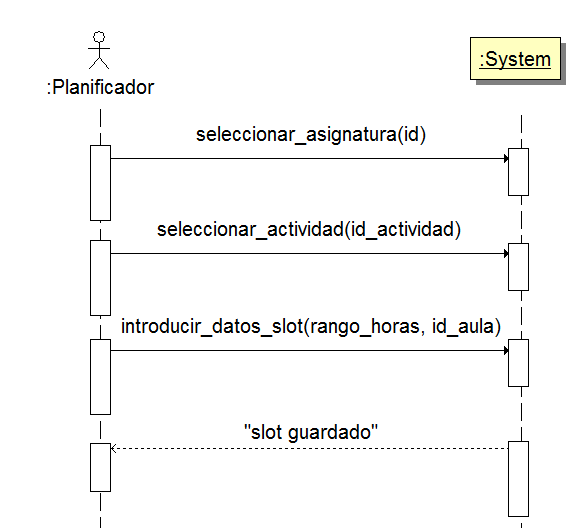
\includegraphics[scale=0.5]{./secuencia-ubicar-slot.png}
  \end{center}
\caption{Diagrama de secuencia del caso de uso Ubicar slot de horario}
\end{figure}

\subsubsection{Contrato de la operación: seleccionar\_actividad}
\begin{itemize}
\item {\bf Responsabilidades:} Seleccionar una actividad para introducirla en el horario
\item {\bf Referencias cruzadas:} Caso de uso {\em ubicar slot de horario}.
\item {\bf Precondiciones:} La asignatura elegida dispone de horas en el plan docente para esa actividad.
\item {\bf Postcondiciones:} Se devuelve una instancia de un Slot de horario para esa asignatura y actividad.
\end{itemize}

\subsubsection{Contrato de la operación: introducir\_datos\_slot}
\begin{itemize}
\item {\bf Responsabilidades:} Ubicar en el horario un slot de una actividad de una asignatura.
\item {\bf Referencias cruzadas:} Caso de uso {\em ubicar slot de horario}
\item {\bf Precondiciones:} Si el slot es de teoría no se solapa con otro slot. No se debe solapar con otro slot con el mismo id\_aula.
\item {\bf Postcondiciones:} El slot queda ubicado en el horario.
\end{itemize}

\subsection{Caso de uso: Editar horario tipo}
\begin{figure}[H] 
  \label{comportamiento-editar-tipo} 
	\begin{center}
    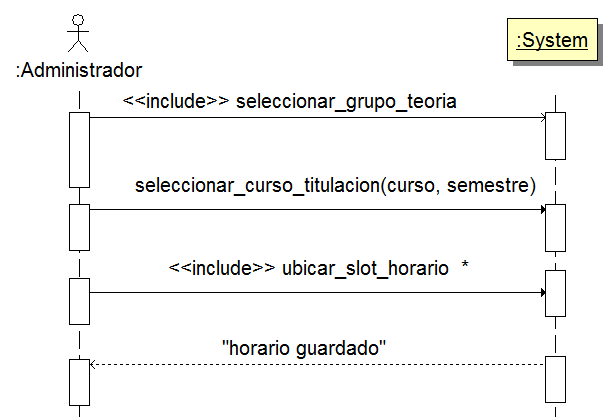
\includegraphics[scale=0.5]{./secuencia-editar-tipo.png}
  \end{center}
\caption{Diagrama de secuencia del caso de uso Editar horario tipo}
\end{figure}

\subsubsection{Contrato de la operación: seleccionar\_curso\_titulacion}
\begin{itemize}
\item {\bf Responsabilidades:} Seleccionar una instancia del Horario
\item {\bf Referencias cruzadas:} Caso de uso {\em editar horario tipo}, Caso de uso {\em editar horario semana inicial}.
\item {\bf Precondiciones:} El curso está dentro de los que tiene la titulación.
\item {\bf Postcondiciones:} Se devuelve una instancia de Horario (o se crea una si no existe).
\end{itemize}

\subsection{Caso de uso: Comprobar grupo de teoría}
\begin{figure}[H] 
  \label{comportamiento-comprobar-grupo} 
	\begin{center}
    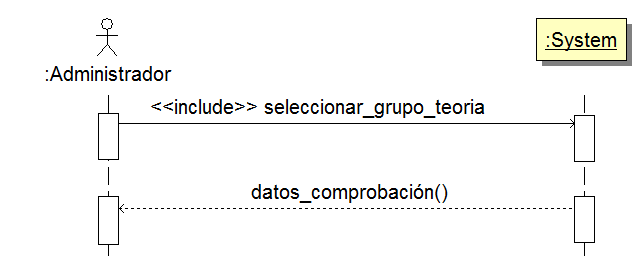
\includegraphics[scale=0.5]{./secuencia-comprobar-grupo.png}
  \end{center}
\caption{Diagrama de secuencia del caso de uso Comprobar grupo de teoría}
\end{figure}

\subsection{Caso de uso: Crear aula}

\begin{figure}[H] 
  \label{comportamiento-crear-aula} 
	\begin{center}
    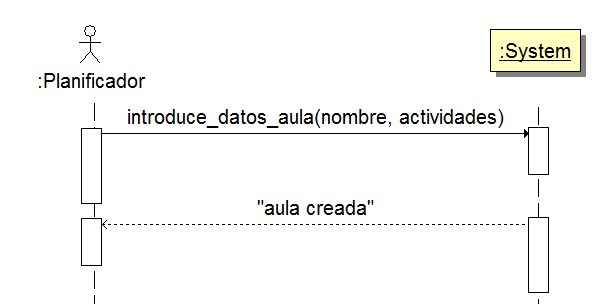
\includegraphics[scale=0.5]{./secuencia-crear-aula.png}
  \end{center}
\caption{Diagrama de secuencia del caso de uso Crear aula}
\end{figure}

\subsubsection{Contrato de la operación: introducir\_datos\_aula}
\begin{itemize}
\item {\bf Responsabilidades:} Crear un aula en el sistema.
\item {\bf Referencias cruzadas:} Caso de uso {\em crear aula}, Caso de uso {\em Editar aula}.
\item {\bf Precondiciones:} No existe ningún aula en el sistema con A.nombre = nombre.
\item {\bf Postcondiciones:} Se crea una instancia A de Aula con A.nombre = nombre y A.actividades = actividades.
\end{itemize}

\subsection{Caso de uso: Borrar aula}
\begin{figure}[H] 
  \label{comportamiento-borrar-aula} 
	\begin{center}
    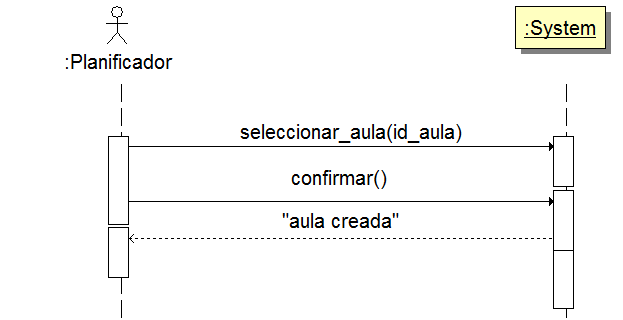
\includegraphics[scale=0.5]{./secuencia-borrar-aula.png}
  \end{center}
\caption{Diagrama de secuencia del caso de uso Borrar aula}
\end{figure}

\subsubsection{Contrato de la operación: seleccionar\_aula}
\begin{itemize}
\item {\bf Responsabilidades:} Seleccionar un aula para borrarla o editarla.
\item {\bf Referencias cruzadas:} Caso de uso {\em borrar aula}, Caso de uso {\em editar aula}.
\item {\bf Precondiciones:} Existe un aula en el sistema con A.id\_aula = id\_aula.
\item {\bf Postcondiciones:} Se devuelve una instancia A de aula con A.id\_aula = id\_aula.
\end{itemize}

\subsection{Caso de uso: Editar aula}
\begin{figure}[H] 
  \label{comportamiento-editar-aula} 
	\begin{center}
    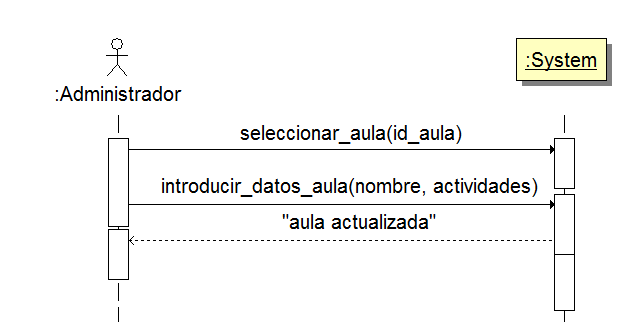
\includegraphics[scale=0.5]{./secuencia-editar-aula.png}
  \end{center}
\caption{Diagrama de secuencia del caso de uso Editar aula}
\end{figure}
% Plantilla para contratos de operaciones
